%\documentclass[12pt]{article}

\questionheader{ex:s2.7}


%%%%%%%%%%%%%%%%%%
\subsection*{\Conceptual}
%%%%%%%%%%%%%%%%%%

%%%%%%%%%%%%%%%%%%%%%%%%%%%%
%\Instructions{Questions~\ref{prob_s1.0first} through \ref{prob_s1.0last} provide practice with.}
%%%%%%%%%%%%%%%%%%%%


%%%%%%%%%%%%%%%%%%%%%%%%%%%%%%%%
\begin{question}[M200 2008A] %1a
Find the directional derivative of $f(x,y,z) = e^{xyz}$ in the $\llt 0,1,1\rgt$ 
direction at the point $(0,1,1)$.
\end{question}

%\begin{hint}
%
%\end{hint}

\begin{answer}
$0$
\end{answer}

\begin{solution}
The partial derivatives, at a general point $(x,y,z)$ and
also at the point of interest $(0,1,1)$, are
\begin{alignat*}{3}
f_x(x,y,z)&=yz e^{xyz}\qquad &
   f_x(0,1,1)&= 1 \\
f_y(x,y,z)&=xz e^{xyz}\qquad &
   f_y(0,1,1)&= 0 \\
f_z(x,y,z)&=xy e^{xyz}\qquad &
   f_z(0,1,1)&= 0 
\end{alignat*}
So $\vnabla f(0,1,1) =\llt 1,0,0\rgt$ and the specified directional derivative
is
\begin{align*}
D_{\frac{\llt 0,1,1\rgt}{\sqrt{2}}}f(0,1,1)
=\llt 1,0,0\rgt\cdot\frac{\llt 0,1,1\rgt}{\sqrt{2}}
=0
\end{align*}
\end{solution}

%%%%%%%%%%%%%%%%%%%%%%%%%%%%%%%%
\begin{question}[M200 2008A] %1d
Find $\vnabla\big(y^2 + \sin(xy)\big)$.
\end{question}

%\begin{hint}
%
%\end{hint}

\begin{answer}
$y\cos(xy)\,\hi +  [2y + x\cos(xy)]\,\hj$
\end{answer}

\begin{solution}
In two dimensions, write $g(x,y) = y^2+\sin(xy)$. Then
\begin{align*}
\vnabla g =\llt g_x\,,\,g_y\rgt
          =\llt y\cos(xy)\,,\, 2y + x\cos(xy) \rgt 
\end{align*}
In three dimensions, write $g(x,y,z) = y^2+\sin(xy)$. Then
\begin{align*}
\vnabla g =\llt g_x\,,\,g_y\,,\,g_z\rgt
          =\llt y\cos(xy)\,,\, 2y + x\cos(xy)\,,\, 0 \rgt 
\end{align*}
\end{solution}

%%%%%%%%%%%%%%%%%%
\subsection*{\Procedural}
%%%%%%%%%%%%%%%%%%

%%%%%%%%%%%%%%%%%%%%%%%%%%%%%%%%
\begin{question}
Find the rate of change of the given function at the given point in
the given direction. 
\begin{enumerate}[(a)]
\item
$f(x,y)=3x-4y$ at the point $(0,2)$ in the direction $-2\hi$.
\item
$f(x,y,z)=x^{-1}+y^{-1}+z^{-1}$ at $(2,-3,4)$ in the direction
$\hi+\hj+\hk$.
\end{enumerate}
\end{question}

%\begin{hint}
%
%\end{hint}

\begin{answer}
(a) $-3$\qquad
(b) $-\frac{61}{144\sqrt{3}}\approx-0.2446$
\end{answer}

\begin{solution}
(a)
The gradient of $f$ is $\vnabla f(x,y)=\llt 3,-4\rgt$. So the specified rate of change is
\begin{equation*}
\llt 3,-4\rgt\cdot\frac{\llt -2,0\rgt}{|\llt -2,0\rgt|}=-3
\end{equation*}

(b)
The gradient of $f$ is
  $\vnabla f(x,y,z)=\llt -x^{-2},-y^{-2},-z^{-2}\rgt$. In particular,
the gradient of $f$ at the point $(2,-3,4)$ is
$\vnabla f(2,-3,4)=\llt -\frac{1}{4},-\frac{1}{9},-\frac{1}{16}\rgt$.
So the specified rate of change is
\begin{equation*} 
\llt -\frac{1}{4},-\frac{1}{9},-\frac{1}{16}\rgt\cdot
        \frac{\llt 1,1,1\rgt}{\sqrt{3}}=
        -\frac{61}{144\sqrt{3}}\approx-0.2446
\end{equation*}
\end{solution}

%%%%%%%%%%%%%%%%%%%%%%%%%%%%%%%%
\begin{question}
 In what directions at the point $(2,0)$ does the function $f(x,y)=xy$
have the specified rates of change? 
\begin{enumerate}[(a)]
\item 
$-1$
\item
$-2$
\item
$-3$
\end{enumerate}
\end{question}

\begin{hint}
The rate of change in the direction that makes angle $\theta$ with
respect to the $x$-axis, that is, in the direction 
$\llt \cos\theta,\sin\theta\rgt$ is 
$
\llt \cos\theta,\sin\theta\rgt \cdot\vnabla f(2,0)
$.
\end{hint}


\begin{answer}
(a) $\llt\pm\frac{\sqrt{3}}{2} ,-\frac{1}{2} \rgt$\qquad
(b) $\llt 0 ,-1 \rgt$ \qquad
(c) No direction works!

\end{answer}

\begin{solution}
The gradient of $f(x,y)$ is $\vnabla f(x,y)=\llt y,x\rgt$. In particular,
the gradient of $f$ at the point $(2,0)$ is
$\vnabla f(2,0)=\llt 0,2 \rgt$. So the rate of change in the direction 
that makes angle $\theta$ with respect to the $x$-axis, that is, 
in the direction 
$\llt \cos\theta,\sin\theta\rgt$ is 
\begin{equation*}
\llt \cos\theta,\sin\theta\rgt \cdot\vnabla f(2,0)
=\llt \cos\theta,\sin\theta\rgt \cdot\llt 0, 2\rgt =2\sin\theta
\end{equation*}

(a) To get a rate $-1$, we need
\begin{equation*}
 \sin\theta=-\frac{1}{2} \implies \theta=-30^\circ,\ -150^\circ
\end{equation*}
So the desired directions are
\begin{equation*}
\llt \cos\theta,\sin\theta\rgt
=\llt\pm\frac{\sqrt{3}}{2} ,-\frac{1}{2} \rgt
\end{equation*}

(b) To get a rate $-2$, we need
\begin{equation*}
 \sin\theta=-1 \implies \theta=-90^\circ
\end{equation*}
So the desired direction is
\begin{equation*}
\llt \cos\theta,\sin\theta\rgt
=\llt 0 ,-1 \rgt
\end{equation*}

(c) To get a rate $-3$, we need
\begin{equation*}
 \sin\theta=-\frac{3}{2}
\end{equation*}
No $\theta$ obeys this, since $-1\le\sin\theta\le 1$ for all $\theta$. 
So no direction works!
\end{solution}

%%%%%%%%%%%%%%%%%%%%%%%%%%%%%%%%
\begin{question}
Find $\vnabla f(a,b)$ given the directional derivatives
\begin{equation*}
D_{(\hi+\hj)/\sqrt{2}}f(a,b)=3\sqrt{2}\qquad
D_{(3\hi-4\hj)/5}f(a,b)=5
\end{equation*}
\end{question}

\begin{hint}
Denote $\vnabla f(a,b)=\llt \al,\be\rgt$.
\end{hint}

\begin{answer}
$\vnabla f(a,b)=\llt 7,-1\rgt$
\end{answer}

\begin{solution}
 Denote $\vnabla f(a,b)=\llt \al,\be\rgt$. We are told that
\begin{alignat*}{5}
\llt\al,\be\rgt\cdot\llt\frac{1}{\sqrt{2}},\frac{1}{\sqrt{2}}\rgt&=3\sqrt{2} &
&\quad\text{or}\quad &
\al+\be&=6\\
\llt\al,\be\rgt\cdot\llt\frac{3}{5},-\frac{4}{5}\rgt&=5 &
&\quad\text{or}\quad &
3\al-4\be&=25
\end{alignat*}
Adding 4 times the first equation to the second equation gives $7\al=49$.
Substituting $\al=7$ into the first equation gives $\be=-1$. So
$\vnabla f(a,b)=\llt 7,-1\rgt$.
\end{solution}


%%%%%%%%%%%%%%%%%%%%%%%%%%%%%%%%
\begin{question}[M200 2005D] %3
You are standing at a location where the surface of the earth is smooth. 
The slope in the southern direction is $4$ and the slope in the south--eastern direction is $\sqrt{2}$. Find the slope in the eastern direction.
\end{question}

\begin{hint}
Use a coordinate system with the positive $y$--axis pointing 
north, with the positive $x$--axis pointing east and with our current
location being $x=y=0$. Denote by $z(x,y)$ the elevation of the 
earth's surface at $(x,y)$. Express the various slopes in terms of
$\vnabla z(0,0)$.
\end{hint}

\begin{answer}
$-2$
\end{answer}

\begin{solution}
Use a coordinate system with the positive $y$--axis pointing 
north, with the positive $x$--axis pointing east and with our current
location being $x=y=0$. Denote by $z(x,y)$ the elevation of the 
earth's surface at $(x,y)$. We are told that
\begin{align*}
\vnabla z(0,0)\cdot(-\hj) &= 4 \\
\vnabla z(0,0)\cdot\left(\frac{\hi-\hj}{\sqrt{2}}\right) &= \sqrt{2} 
\end{align*}
The first equation implies that $z_y(0,0)=-4$ and the second equation 
implies that
\begin{align*}
\frac{z_x(0,0)-z_y(0,0)}{\sqrt{2}}=\sqrt{2}
\implies
z_x(0,0)=z_y(0,0)+2 = -2
\end{align*}
So the slope in the eastern direction is
\begin{align*}
\vnabla z(0,0)\cdot\hi = z_x(0,0) = -2
\end{align*}

\end{solution}

%%%%%%%%%%%%%%%%%%%%%%%%%%%%%%%%
\begin{question}[M200 2006A] %2
Assume that the directional derivative of $w = f(x,y,z)$ at a point $P$ 
is a maximum in the direction of the vector $2\hi - \hj + \hk$, and 
the value of the directional derivative in that direction is $3\sqrt{6}$.
\begin{enumerate}[(a)]
\item
Find the gradient vector of $w = f(x,y,z)$ at $P$. 
\item
Find the directional derivative of $w = f(x,y,z)$ at $P$ in the 
direction of the vector $\hi + \hj$
\end{enumerate}
\end{question}

%\begin{hint}
%
%\end{hint}

\begin{answer}
(a) $6\hi - 3\hj + 3\hk$\qquad
(b) $\frac{3}{\sqrt{2}}$
\end{answer}

\begin{solution}
(a)  Use $\vnabla f(P)$ to denote the gradient vector of $f$
at $P$. We are told that
\begin{itemize}
\item
directional derivative  of $f$ at $P$ is a maximum in the direction 
$2\hi - \hj + \hk$, which implies that $\vnabla f(P)$ is parallel
to $2\hi - \hj + \hk$, and
\item
the magnitude of the directional derivative in that direction is $3\sqrt{6}$,
which implies that $|\vnabla f(P)|=3\sqrt{6}$.
\end{itemize}
So
\begin{align*}
\vnabla f(P) = 3\sqrt{6} \frac{2\hi - \hj + \hk}{|2\hi - \hj + \hk|}
             = 6\hi - 3\hj + 3\hk
\end{align*}

(b) The directional derivative of $f$ at $P$ in the direction $\hi+\hj$ is
\begin{equation*}
\vnabla f(P) \cdot\frac{\hi+\hj}{|\hi+\hj|}
=\frac{1}{\sqrt{2}}\big(6\hi - 3\hj + 3\hk\big)\cdot\big(\hi+\hj\big)
=\frac{3}{\sqrt{2}}
\end{equation*}
\end{solution}

%%%%%%%%%%%%%%%%%%%%%%%%%%%%%%%%
\begin{question}[M200 2006D] %2
A hiker is walking on a mountain with height above the $z = 0$ plane given by
\begin{equation*}
z = f(x,y) = 6 - xy^2 
\end{equation*}
The positive $x$--axis points east and the positive $y$--axis points north, 
and the hiker starts from the point $P(2, 1, 4)$.
\begin{enumerate}[(a)]
\item
In what direction should the hiker proceed from $P$ to ascend 
along the steepest path? What is the slope of the path?
\item
Walking north from $P$, will the hiker start to ascend or descend? 
What is the slope?
\item
In what direction should the hiker walk from $P$ to remain at the same height?
\end{enumerate}
\end{question}

%\begin{hint}
%
%\end{hint}

\begin{answer}
(a) The path of steepest ascent is in the direction 
$-\frac{1}{\sqrt{17}}\llt 1\,,\, 4\rgt$, which is a little
west of south. The slope is
$
|\vnabla f(2,1)| = |\llt -1\,,\, -4\rgt| = \sqrt{17}
$.

(b) So the hiker descends with slope $4$.

(c) $\pm\frac{1}{\sqrt{17}}\llt 4, -1\rgt$
\end{answer}

\begin{solution}
(a) The gradient of $f$ at $(x,y)=(2,1)$ is
\begin{align*}
\vnabla f(2,1) = \llt -y^2\,,\,-2xy \rgt\Big|_{(x,y)=(2,1)}
               = \llt -1\,,\, -4\rgt
\end{align*}
So the path of steepest ascent is in the direction 
$-\frac{1}{\sqrt{17}}\llt 1\,,\, 4\rgt$, which is a little
west of south. The slope is
\begin{equation*}
|\vnabla f(2,1)| = |\llt -1\,,\, -4\rgt| = \sqrt{17}
\end{equation*}

(b) The directional derivative in the north direction is
\begin{equation*}
D_{\llt 0,1\rgt}f(2,1) = \vnabla f(2,1)\cdot\llt 0,1\rgt
               = \llt -1\,,\, -4\rgt \cdot \llt 0,1\rgt = -4
\end{equation*}
So the hiker descends with slope $|-4|=4$.

(c) To contour, i.e. remain at the same height, the hiker should walk
in a direction perpendicular to $\vnabla f(2,1)= \llt -1\,,\, -4\rgt$.
Two unit vectors perpendicular to $\llt -1\,,\, -4\rgt$
are $\pm\frac{1}{\sqrt{17}}\llt 4, -1\rgt$.
\end{solution}

%%%%%%%%%%%%%%%%%%%%%%%%%%%%%%%%
\begin{question}
Two hikers are climbing a (small) mountain whose height is 
$\ z=1000-2x^2-3y^2.$ 
They start at $\ (1,1,995)\ $ and follow the path of steepest ascent. Their
$(x,y)$ coordinates obey $\ y=ax^b\ $ for some constants $a, b$. 
Determine $a$ and $b$.
\end{question}

\begin{hint}
In order for $y=ax^b$ to give the $(x,y)$ coordinates of the
path of steepest ascent,  the tangent vector to $y=ax^b$ must be parallel
to the height gradient $\vnabla h(x,y)$ at all points on $y=ax^b$.
Also, don't forget that $(1,1)$ must be on $y=ax^b$.
\end{hint}

\begin{answer}
$a=1$, $b=\frac{3}{2}$
\end{answer}

\begin{solution}
 The gradient of $h(x,y)=1000-2x^2-3y^2$ is 
$\vnabla h(x,y)=(-4x,-6y)$. This gradient (which points in the direction
of steepest ascent) must be parallel to the tangent to $y=ax^b$ at all
points on $y=ax^b$. A tangent to $y=ax^b$ is $\llt 1,\diff{y}{x}\rgt
=\llt 1, abx^{b-1}\rgt$. 
\begin{equation*}
\llt -4x,-6y\rgt \parallel \llt 1, abx^{b-1}\rgt
\implies \frac{abx^{b-1}}{1}=\frac{-6y}{-4x}
\implies \frac{3}{2}y=abx^b
\end{equation*}
This is true at all points on $y=ax^b$ if and only if $b=\frac{3}{2}$.
As $(1,1)$ must also be on $y=ax^b$, we need $1=a1^b$, which forces
$a=1$, $b=\frac{3}{2}$. Here is a contour map showing the hiking trail.
\begin{center}
     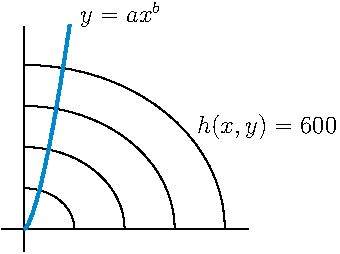
\includegraphics{hiker.pdf}
\end{center}
\end{solution}



%%%%%%%%%%%%%%%%%%%%%%%%%%%%%%%%
\begin{question}[M200 2007A] %3
A mosquito is at the location $(3, 2, 1)$ in $\bbbr^3$. 
She knows that the temperature $T$ near there is given by 
$T = 2x^2 + y^2 - z^2$.
\begin{enumerate}[(a)]
\item
She wishes to stay at the same temperature, but must fly in some 
initial direction. Find a direction in which the initial rate of 
change of the temperature is $0$.

\item
 If you and another student both get correct answers in part (a), 
must the directions you give be the same? Why or why not?

\item 
What initial direction or directions would suit the mosquito if 
she wanted to cool down as fast as possible?
\end{enumerate}
\end{question}

%\begin{hint}
%
%\end{hint}

\begin{answer}
(a) Any nonzero $\llt a\,,\,b\,,\,c\rgt$ that obeys $12a+4b-2c=0$
is an allowed direction. Four allowed unit vectors are
$\pm\frac{\llt 0\,,\,1\,,\,2\rgt}{\sqrt{5}}$ and
$\pm\frac{\llt 1\,,\,-3\,,\,0\rgt}{\sqrt{10}}$.

(b) No they need not be the same. Four different explicit directions
     were given in part (a).

(c) $-\frac{\llt 6\,,\,2\,,\,-1\rgt}{\sqrt{41}}$
\end{answer}

\begin{solution}
(a) The temperature gradient at $(3,2,1)$ is
\begin{align*}
\vnabla T(3,2,1) = \llt 4x\,,\,2y\,,\,-2z\rgt\Big|_{(x,y,z)=(3,2,1)}
                 = \llt 12\,,\,4\,,\,-2\rgt
\end{align*}
She wishes to fly in a direction that is perpendicular to $\vnabla T(3,2,1)$.
That is, she wishes to fly in a direction $\llt a\,,\,b\,,\,c\rgt$
that obeys
\begin{equation*}
0 = \llt 12\,,\,4\,,\,-2\rgt\cdot \llt a\,,\,b\,,\,c\rgt
  = 12a+4b-2c
\end{equation*}
Any nonzero $\llt a\,,\,b\,,\,c\rgt$ that obeys $12a+4b-2c=0$
is an allowed direction. Four allowed unit vectors are
$\pm\frac{\llt 0\,,\,1\,,\,2\rgt}{\sqrt{5}}$ and
$\pm\frac{\llt 1\,,\,-3\,,\,0\rgt}{\sqrt{10}}$.

(b) No they need not be the same. Four different explicit directions
     were given in part (a).

(c) To cool down as quickly as possible, she should move in the direction
    opposite to the temperature gradient. A unit vector in that direction is 
    $-\frac{\llt 6\,,\,2\,,\,-1\rgt}{\sqrt{41}}$.
\end{solution}

%%%%%%%%%%%%%%%%%%%%%%%%%%%%%%%%
\begin{question}[M200 2008D] %4

\end{question}
The air temperature $T(x,y,z)$ at a location $(x,y,z)$ is given by:
\begin{equation*}
T(x,y,z) = 1 + x^2 + yz.
\end{equation*}
\begin{enumerate}[(a)]
\item
A bird passes through $(2,1,3)$ travelling towards $(4,3,4)$ with speed $2$.
At what rate does the air temperature it experiences change at this instant?

\item
If instead the bird maintains constant altitude ($z = 3$) as it passes
through $(2,1,3)$ while also keeping at a fixed air temperature, $T = 8$, 
what are its two possible directions of travel?
\end{enumerate}
%\begin{hint}
%
%\end{hint}

\begin{answer}
(a) $10$\qquad
(b) $\pm \frac{1}{5}\llt 3\,,-4\,,0\rgt$
\end{answer}

\begin{solution}
The temperature gradient at $(2,1,3)$ is
\begin{align*}
\vnabla T(2,1,3) = \llt 2x\,,\,z\,,\,y \rgt\Big|_{(x,y,z)=(2,1,3)}
                 = \llt 4\,,\,3\,,\,1 \rgt
\end{align*}

(a) The bird is flying in the direction $\llt 4-2\,,\,3-1\,,\,4-3 \rgt
=\llt 2\,,\,2\,,\,1\rgt$ at speed $2$ and so has velocity
$
\vv=2\frac{\llt 2\,,\,2\,,\,1\rgt}{|\llt 2\,,\,2\,,\,1\rgt|}
=\frac{2}{3} \llt 2\,,\,2\,,\,1\rgt
$.
The rate of change of air temperature experienced by the bird at that 
instant is
\begin{align*}
\vnabla T(2,1,3) \cdot\vv
=\frac{2}{3} \llt 4\,,\,3\,,\,1 \rgt \cdot \llt 2\,,\,2\,,\,1\rgt
= 10
\end{align*}

(b) To maintain constant altitude (while not being stationary), 
the bird's direction of travel has to be 
of the form $\llt a\,,\,b\,,\,0\rgt$, for some constants $a$ and $b$,
not both zero. To keep the air temperature fixed, its direction of travel
has to be perpendicular to $\vnabla T(2,1,3)= \llt 4\,,\,3\,,\,1 \rgt$.
So $a$ and $b$ have to obey
\begin{align*}
0 = \llt a\,,\,b\,,\,0\rgt \cdot \llt 4\,,\,3\,,\,1 \rgt
  = 4a+3b
\iff b=-\frac{4}{3}a
\end{align*}
and the direction of travel has to be a nonzero constant times 
$\llt 3\,,-4\,,0\rgt$. The two such unit vectors are 
$\pm \frac{1}{5}\llt 3\,,-4\,,0\rgt$.
\end{solution}

%%%%%%%%%%%%%%%%%%%%%%%%%%%%%%%%
\begin{question}[M200 2009A] %3
Let $f(x,y) = 2x^2 + 3xy + y^2$ be a function of $x$ and $y$.

\begin{enumerate}[(a)]
\item
Find the maximum rate of change of $f(x,y)$ at the point 
$P\left(1, -\frac{4}{3}\right)$.


\item
Find the directions in which the directional derivative of $f(x,y)$ 
at the point $P\left(1, -\frac{4}{3}\right)$ has the value $\frac{1}{5}$.
\end{enumerate}

\end{question}

%\begin{hint}
%
%\end{hint}

\begin{answer}
(a) $\frac{1}{3}$\qquad
(b) $\llt \pm\frac{4}{5}\,,\,\frac{3}{5}\rgt$
\end{answer}

\begin{solution}
We are going to need, in both parts of this question,
the gradient of $f(x,y)$ at $(x,y)=\left(1, -\frac{4}{3}\right)$.
So we find it first.
\begin{alignat*}{3}
f_x(x,y)&=4x+3y\qquad &
f_x(1,-4/3)&=0
\\
f_y(x,y)&=3x+2y\qquad &
f_y(1,-4/3)&=\frac{1}{3}
\end{alignat*}
so $\vnabla f\left(1, -\frac{4}{3}\right) =\llt 0,\frac{1}{3}\rgt$.

(a) The maximum rate of change of $f$ at $P$ is
\begin{align*}
\left|\vnabla f\left(1, -\tfrac{4}{3}\right)\right| 
=\left|\llt 0,\tfrac{1}{3}\rgt\right|
=\tfrac{1}{3}
\end{align*}

(b) If $\llt a,b\rgt$ is a unit vector, the directional derivative of $f$
at $P$ in the direction $\llt a,b\rgt$ is
\begin{align*}
D_{\llt a,b\rgt}f\left(1, -\tfrac{4}{3}\right)
=\vnabla f\left(1, -\tfrac{4}{3}\right)\cdot \llt a,b\rgt
=\llt 0,\tfrac{1}{3}\rgt\cdot \llt a,b\rgt
=\tfrac{b}{3}
\end{align*}
So we need $\frac{b}{3}=\frac{1}{5}$ and hence $b=\frac{3}{5}$.
For $\llt a,b\rgt$ to be a unit vector, we also need
\begin{align*}
a^2+b^2=1
\iff
a^2=1-b^2=1-\frac{3^2}{5^2}=\frac{16}{25}
\iff
a=\pm\frac{4}{5}
\end{align*}
So the allowed directions are $\llt \pm\frac{4}{5}\,,\,\frac{3}{5}\rgt$.
\end{solution}

%%%%%%%%%%%%%%%%%%%%%%%%%%%%%%%%
\begin{question}[M200 2010A] %3
The temperature $T(x, y)$ at a point of the $xy$--plane is given by
\begin{equation*}
T(x, y) = ye^{x^2} 
\end{equation*}
A bug travels from left to right along the curve $y = x^2$ at a speed of $0.01$m/sec. The bug
monitors $T(x, y)$ continuously. What is the rate of change of $T$ as the bug passes through
the point $(1, 1)$?
\end{question}

%\begin{hint}
%
%\end{hint}

\begin{answer}
$\frac{0.04 e}{\sqrt{5}} $
\end{answer}

\begin{solution}
The slope of $y=x^2$ at $(1,1)$ is $\diff{}{x}x^2\Big|_{x=1}=2$.
So a unit vector in the bug's direction of motion is 
$\frac{\llt 1,2\rgt}{\sqrt{5}}$ and the bug's velocity vector is
$\vv=0.01\frac{\llt 1,2\rgt}{\sqrt{5}}$.

The temperature gradient at $(1,1)$ is
\begin{align*}
\vnabla T(1,1) = \llt 2xy e^{x^2}\,,\,e^{x^2}\rgt\Big|_{(x.y)=(1,1)}
               =\llt 2e\,,\,e\rgt
\end{align*}
and the rate of change of $T$ (per unit time) that the bug feels as it 
passes through the point $(1, 1)$ is
\begin{align*}
\vnabla T(1,1)\cdot \vv
=\frac{0.01}{\sqrt{5}} \llt 2e\,,\,e\rgt\cdot \llt 1,2\rgt
=\frac{0.04 e}{\sqrt{5}} 
\end{align*}
\end{solution}

%%%%%%%%%%%%%%%%%%%%%%%%%%%%%%%%
\begin{question}[M200 2010D] %2
Suppose the function $T=F(x,y,z)=3+xy-y^2+z^2-x$ describes the temperature at
a point $(x,y,z)$ in space, with $F(3,2,1)=3$.
\begin{enumerate}[(a)]
\item
Find the directional derivative of $T$ at $(3, 2, 1)$, in the direction of the
point $(0,1,2)$.
\item
At the point $(3, 2, 1)$, in what direction does the temperature
\emph{decrease}  most rapidly?
\item
Moving along the curve given by $x=3e^t$,  $y = 2 \cos t$, $z= \sqrt{1 + t}$, 
find $\diff{T}{t}$, the rate of change of temperature with respect to $t$, at $t = 0$.
\item
Suppose $\hi+5\hj+a\hk$ is a vector that is tangent to the temperature level surface
$T(x, y, z) = 3$ at $(3, 2, 1)$. What is $a$?
\end{enumerate}
\end{question}

%\begin{hint}
%
%\end{hint}

\begin{answer}
(a) $0$\qquad
(b) $ \frac{1}{\sqrt{6}}\llt -1\,,\,1\,,\,-2 \rgt $\qquad
(c) $4$\qquad
(d) $a=2$
\end{answer}

\begin{solution}
(a) 
We are to find the directional derivative in the direction
\begin{equation*}
\llt 0-3\,,\,1-2\,,\,2-1\rgt = \llt -3\,,\,-1\,,\,1\rgt
\end{equation*}
As the gradient of $F$ is
\begin{align*}
\vnabla F(x,y,z) = \llt y-1\,,\,x-2y\,,\,2z \rgt
\end{align*}
the directional derivative is
\begin{align*}
D_{\frac{\llt -3\,,\,-1\,,\,1\rgt}{|\llt -3\,,\,-1\,,\,1\rgt|}}F(3,2,1)
&=\vnabla F(3,2,1)\cdot 
  \frac{\llt -3\,,\,-1\,,\,1\rgt}{|\llt -3\,,\,-1\,,\,1\rgt|} \\
&= \llt 2-1\,,\,3-2(2)\,,\,2(1) \rgt
\cdot   \frac{\llt -3\,,\,-1\,,\,1\rgt}{|\llt -3\,,\,-1\,,\,1\rgt|}
=\llt 1\,,\,-1\,,\,2\rgt \cdot   \frac{\llt -3\,,\,-1\,,\,1\rgt}{\sqrt{11}}\\
&=0
\end{align*}

(b) The temperature decreases most rapidly in the direction opposite the
gradient. A unit vector in that direction is
\begin{align*}
   -\frac{\vnabla F(3,2,1)}{|\vnabla F(3,2,1)|}
=  -\frac{\llt 1\,,\,-1\,,\,2 \rgt}{|\llt 1\,,\,-1\,,\,2 \rgt|}
= \frac{1}{\sqrt{6}}\llt -1\,,\,1\,,\,-2 \rgt 
\end{align*}

(c) The velocity vector at time $0$ is
\begin{align*}
\vv=\llt x'(0)\,,\,y'(0)\,,\,z'(0)\rgt
=\llt 3e^t\,,\,-2\sin t\,,\,\frac{1}{2\sqrt{1+t}}\rgt\Big|_{t=0}
=\llt 3\,,\,0\,,\,\frac{1}{2}\rgt
\end{align*}
So the rate of change of temperature with respect to $t$ at $t=0$ is
\begin{align*}
\vnabla F(3,2,1)\cdot \vv
=\llt 1\,,\,-1\,,\,2 \rgt\cdot 
   \llt 3\,,\,0\,,\,\frac{1}{2}\rgt
=4
\end{align*}

(d) For $\hi+5\hj+a\hk$ to be tangent to the level surface
$F(x, y, z) = 3$ at $(3, 2, 1)$, $\hi+5\hj+a\hk$ must be perpendicular
to  $\vnabla F(3,2,1)$. So
\begin{align*}
0=\llt 1\,,\,5\,,\,a \rgt \cdot \llt 1\,,\,-1\,,\,2 \rgt
 = -4+2a
\end{align*}
So $a=2$.
\end{solution}

%%%%%%%%%%%%%%%%%%%%%%%%%%%%%%%%
\begin{question}[M200 2011A] %4
Let
\begin{align*}
f(x, y, z) &= (2x + y)e^{-(x^2 +y^2 +z^2)} \\
g(x, y, z) &= xz + y^2 + yz + z^2 
\end{align*}
\begin{enumerate}[(a)]
\item
Find the gradients of $f$ and $g$ at $(0,1,-1)$.
\item
A bird at $(0,1,-1)$ flies at speed $6$ in the direction in which $f(x, y, z)$ increases 
most rapidly. As it passes through $(0,1,-1)$, how quickly does $g(x, y, z)$ appear (to the bird) 
to be changing?
\item
A bat at $(0,1,-1)$ flies in the direction in which $f (x, y, z)$ and $g(x, y, z)$ do not change,
but $z$ increases. Find a vector in this direction.
\end{enumerate}
\end{question}

%\begin{hint}
%
%\end{hint}

\begin{answer}
(a) $\vnabla f(0,1,-1) =e^{-2}\llt 2,-1,2\rgt$, 
    $\vnabla g(0,1,-1) =\llt -1,1,-1\rgt$\qquad
(b) $10$

(c) Any vector which is a (strictly)
positive constant times $\llt -1 \,,\, 0 \,,\, 1 \rgt$ is fine.
\end{answer}

\begin{solution}
(a) The first order partial derivatives of $f$ and $g$ are
\begin{alignat*}{3}
\pdiff{f}{x}(x,y,z)&=  2e^{-(x^2 +y^2 +z^2)} -2x(2x + y)e^{-(x^2 +y^2 +z^2)}
&\quad\implies \pdiff{f}{x}(0,1,-1)&=2e^{-2} \\
\pdiff{f}{y}(x,y,z)&=  e^{-(x^2 +y^2 +z^2)} -2y(2x + y)e^{-(x^2 +y^2 +z^2)}
&\quad\implies \pdiff{f}{y}(0,1,-1)&=-e^{-2} \\
\pdiff{f}{z}(x,y,z)&=  -2z(2x + y)e^{-(x^2 +y^2 +z^2)}
&\quad\implies \pdiff{f}{z}(0,1,-1)&=2e^{-2} 
\\
\pdiff{g}{x}(x,y,z)&=  z
&\quad\implies \pdiff{g}{x}(0,1,-1)&=-1 \\
\pdiff{g}{y}(x,y,z)&=  2y+z
&\quad\implies \pdiff{g}{y}(0,1,-1)&= 1 \\
\pdiff{g}{z}(x,y,z)&=  x+y+2z
&\quad\implies \pdiff{g}{z}(0,1,-1)&=-1
\end{alignat*}
so that gradients are
\begin{equation*}
\vnabla f(0,1,-1) =e^{-2}\llt 2,-1,2\rgt\qquad
\vnabla g(0,1,-1) =\llt -1,1,-1\rgt
\end{equation*}

(b) The bird's velocity is the vector of length $6$ in the direction of
$\vnabla f(0,1,-1)$, which is
\begin{equation*}
\vv= 6\frac{\llt 2,-1,2\rgt}{|\llt 2,-1,2\rgt|}
=\llt 4,-2,4\rgt
\end{equation*}
The rate of change of $g$ (per unit time) seen by the bird is
\begin{align*}
\vnabla g(0,1,-1) \cdot \vv
=\llt -1,1,-1\rgt \cdot \llt 4,-2,4\rgt
= -10
\end{align*}

(c) The direction of flight for the bat has to be perpendicular to both
$\vnabla f(0,1,-1) =e^{-2}\llt 2,-1,2\rgt$ and 
$\vnabla g(0,1,-1) =\llt -1,1,-1\rgt$. Any vector which is a non zero constant
times
\begin{align*}
\llt 2,-1,2\rgt \times \llt -1,1,-1\rgt
    =\det\left[\begin{matrix}
            \hi  &  \hj  &  \hk \\
             2   &  -1   &   2 \\
            -1   &   1   &  -1 
            \end{matrix}\right]
=\llt -1 \,,\, 0 \,,\, 1 \rgt
\end{align*}
is perpendicular to both $\vnabla f(0,1,-1)$ and 
$\vnabla g(0,1,-1)$. In addition, the direction of flight for the bat
must have a positive $z$--component. So any vector which is a (strictly)
positive constant times $\llt -1 \,,\, 0 \,,\, 1 \rgt$ is fine.
\end{solution}

%%%%%%%%%%%%%%%%%%%%%%%%%%%%%%%%
\begin{question}[M200 2011D] %3
A bee is flying along the curve of intersection of the surfaces $3z + x^2 + y^2 = 2$ and
$z = x^2 - y^2$ in the direction for which $z$ is increasing. At time $t = 2$, the bee passes
through the point $(1, 1, 0)$ at speed $6$.
\begin{enumerate}[(a)]
\item
Find the velocity (vector) of the bee at time $t = 2$.
\item
The temperature $T$ at position $(x, y, z)$ at time $t$ is given by $T = xy - 3x+2yt+z$.
Find the rate of change of temperature experienced by the bee at time $t = 2$.
\end{enumerate}
\end{question}

%\begin{hint}
%
%\end{hint}

\begin{answer}
(a) $\vv = \llt -2 \,,\, -4 \,,\, 4 \rgt$\qquad
(b) $-10$
\end{answer}

\begin{solution}
(a) Let's use $\vv$ to denote the bee's velocity vector at time $t=2$.
\begin{itemize}
\item 
The bee's direction of motion is tangent to the curve.
That tangent is perpendicular to both the normal vector to
$3z + x^2 + y^2 = 2$ at $(1,1,0)$, which is 
\begin{equation*}
\llt 2x\,,\,2y\,,\,3\rgt\Big|_{(x,y,z)=(1,1,0)} = \llt 2\,,\,2\,,\,3\rgt
\end{equation*}
and the normal vector to $z = x^2 - y^2$ at $(1,1,0)$, which is 
\begin{equation*}
\llt 2x\,,\,-2y\,,\,-1\rgt\Big|_{(x,y,z)=(1,1,0)} = \llt 2\,,\,-2\,,\,-1\rgt
\end{equation*}
So $\vv$ has to be some constant times
\begin{align*}
\llt 2\,,\,2\,,\,3\rgt \times \llt 2\,,\,-2\,,\,-1\rgt
    =\det\left[\begin{matrix}
            \hi  &  \hj  &  \hk \\
            2    &   2   &    3 \\
            2    &  -2   &   -1 
            \end{matrix}\right]
=\llt 4 \,,\, 8 \,,\, -8 \rgt
\end{align*}
or, equivalently, some constant times $\llt 1 \,,\, 2 \,,\, -2 \rgt$.

\item
Since the $z$--component of $\vv$ has to be positive,
$\vv$ has to be a positive constant times 
$\llt -1 \,,\, -2 \,,\, 2 \rgt$.

\item
Since the speed has to be $6$,  $\vv$ has to have length $6$.
\end{itemize}
As $|\llt -1 \,,\, -2 \,,\, 2 \rgt|=3$
\begin{equation*}
\vv = 2\llt -1 \,,\, -2 \,,\, 2 \rgt
    =\llt -2 \,,\, -4 \,,\, 4 \rgt
\end{equation*}

(b) \emph{Solution 1}:\ \ \ 
Suppose that the bee is at $\big(x(t),y(t),z(t)\big)$ at time $t$.
Then the temperature that the bee feels at time $t$ is
\begin{align*}
T\big(x(t),y(t),z(t),t\big) = x(t) y(t) -3x(t) +2y(t) t +z(t)
\end{align*}
Then the rate of change of temperature (per unit time) felt by the bee at time
$t=2$ is
\begin{align*}
\diff{}{t}T\big(x(t),y(t),z(t),t\big)\Big|_{t=2}
&=x'(2)y(2) + x(2)y'(2) -3x'(2) +2y'(2)2+2y(2) +z'(2) \\
\end{align*}
Recalling that, at time $t=2$, the bee is at $(1,1,0)$ and has velocity
$\llt -2 \,,\, -4 \,,\, 4 \rgt$
\begin{align*}
\diff{}{t}T\big(x(t),y(t),z(t),t\big)\Big|_{t=2}
&=(-2)(1) + (1)(-4) -3(-2) +2(-4)2+2(1) +4 \\
&=-10
\end{align*}


(b) \emph{Solution 2}:\ \ \ 
Suppose that the bee is at $\big(x(t),y(t),z(t)\big)$ at time $t$.
Then the temperature that the bee feels at time $t$ is
\begin{align*}
T\big(x(t),y(t),z(t),t\big) 
\end{align*}
By the chain rule, the rate of change of temperature (per unit time) 
felt by the bee at time $t=2$ is
\begin{align*}
\diff{}{t}T\big(x(t),y(t),z(t),t\big)\Big|_{t=2}
&=\bigg[\pdiff{T}{x}\big(x(t),y(t),z(t),t\big)\,x'(t)
      +\pdiff{T}{y}\big(x(t),y(t),z(t),t\big)\,y'(t) \\&\hskip0.5in
      +\pdiff{T}{z}\big(x(t),y(t),z(t),t\big)\,z'(t)
      +\pdiff{T}{t}\big(x(t),y(t),z(t),t\big)\bigg]_{t=2}
\end{align*}
Recalling that $T = xy - 3x+2yt+z$, we have
\begin{align*}
\diff{}{t}T\big(x(t),y(t),z(t),t\big)\Big|_{t=2}
&=[y(2)-3]x'(2) + [x(2)+2\times 2]y'(2) +z'(2) +2y(2)  
\end{align*}
Also recalling that, at time $t=2$, the bee is at $(1,1,0)$ and has velocity
$\llt -2 \,,\, -4 \,,\, 4 \rgt$
\begin{align*}
\diff{}{t}T\big(x(t),y(t),z(t),t\big)\Big|_{t=2}
&=[-2](-2) + [5](-4) +4  +2 \\
&=-10
\end{align*}
\end{solution}

%%%%%%%%%%%%%%%%%%%%%%%%%%%%%%%%
\begin{question}[M200 2012a] %4
The temperature at a point $(x, y, z)$ is given by 
$T(x, y, z) = 5e^{-2x^2-y^2-3z^2}$, 
where $T$ is measured in centigrade and $x$, $y$, $z$ in meters.
\begin{enumerate}[(a)]
\item
Find the rate of change of temperature at the point $P(1, 2, -1)$ in the 
direction toward the point $(1, 1, 0)$.
\item
In which direction does the temperature decrease most rapidly?
\item
Find the maximum rate of decrease at $P$.
\end{enumerate}
\end{question}

%\begin{hint}
%
%\end{hint}

\begin{answer}
(a) $25\,\sqrt{2}\,e^{-9}$\qquad
(b) $\frac{\llt 2,2,-3\rgt}{\sqrt{17}}$\qquad
(c) $-10\sqrt{17} e^{-9}$
\end{answer}

\begin{solution}
(a) We are to find the rate of change of $T(x,y,z)$ at $(1, 2, -1)$
in the direction $\llt 1, 1, 0\rgt - \llt 1, 2, -1\rgt = \llt 0,-1,1 \rgt$.
That rate of change (per unit distance) is the directional derivative
\begin{align*}
D_{\frac{\llt 0,-1,1 \rgt}{\sqrt{2}}} T(1,2,-1)
=\vnabla T(1,2,-1)\cdot \frac{\llt 0,-1,1 \rgt}{\sqrt{2}}
\end{align*}
As
\begin{align*}
\pdiff{T}{x}(x,y,z)&= -20 x\,e^{-2x^2-y^2-3z^2} &
   \pdiff{T}{x}(1,2,-1)&= -20\, e^{-9} \\
\pdiff{T}{y}(x,y,z)&= -10 y\,e^{-2x^2-y^2-3z^2} &
   \pdiff{T}{y}(1,2,-1)&= -20\, e^{-9} \\
\pdiff{T}{z}(x,y,z)&= -30 z\,e^{-2x^2-y^2-3z^2} &
   \pdiff{T}{z}(1,2,-1)&= 30\, e^{-9} 
\end{align*}
the directional derivative
\begin{align*}
D_{\frac{\llt 0,-1,1 \rgt}{\sqrt{2}}} T(1,2,-1)
=e^{-9}\llt -20,-20,30\rgt\cdot \frac{\llt 0,-1,1 \rgt}{\sqrt{2}}
=\frac{50}{\sqrt{2}}e^{-9} =25\,\sqrt{2}\,e^{-9}
\end{align*}

(b) The direction of maximum rate of decrease is $-\vnabla T(1,2,-1)$.
A unit vector in that direction is $\frac{\llt 2,2,-3\rgt}{\sqrt{17}}$.

(c) The maximum rate of decrease at $P$ is 
  $-|\vnabla T(1,2,-1)|=-10 e^{-9} |\llt -2,-2,3\rgt|
                      = -10\sqrt{17} e^{-9}$.
\end{solution}

%%%%%%%%%%%%%%%%%%%%%%%%%%%%%%%%
\begin{question}[M200 2012D] %5
The directional derivative of a function $w = f(x, y, z)$ at a point $P$ in the direction
of the vector $\hi$ is 2, in the direction of the vector $\hi+\hj$ is $-\sqrt{2}$, and 
in the direction of the vector $\hi+\hj+\hk$ is $-\frac{5}{\sqrt{3}}$. 
Find the direction in which the function $w = f(x, y, z)$  has the
maximum rate of change at the point $P$ . What is this maximum rate of change?
\end{question}

%\begin{hint}
%
%\end{hint}

\begin{answer}
The unit vector in the direction of maximum rate of change is
$\frac{\llt 2\,,\,-4\,,\,-3\rgt}{\sqrt{29}}$.
The maximum rate of change is $\sqrt{29}$.
\end{answer}

\begin{solution}
Denote by $\llt a\,,\,b\,,\,c\rgt$ the gradient of the function $f$ at
$P$. We are told
\begin{align*}
\llt a\,,\,b\,,\,c\rgt \cdot \llt 1\,,\,0\,,\,0\rgt &= 2 \\
\llt a\,,\,b\,,\,c\rgt \cdot \frac{1}{\sqrt{2}}\llt 1\,,\,1\,,\,0\rgt &= -\sqrt{2} \\
\llt a\,,\,b\,,\,c\rgt \cdot \frac{1}{\sqrt{3}}\llt 1\,,\,1\,,\,1\rgt &= -\frac{5}{\sqrt{3}}
\end{align*}
Simplifying
\begin{align*}
a&=2 \\
a+b&=-2 \\
a+b+c&=-5
\end{align*}
From these equations we read off, in order,
$a=2$, $b=-4$ and $c=-3$.
The function $f$ has maximum rate of change at $P$ in the 
direction if the gradient of $f$. The unit vector in that direction is
\begin{equation*}
\frac{\llt 2\,,\,-4\,,\,-3\rgt}{|\llt 2\,,\,-4\,,\,-3\rgt|}
=\frac{\llt 2\,,\,-4\,,\,-3\rgt}{\sqrt{29}}
\end{equation*}
The maximum rate of change is the magnitude of the gradient, which is
$\sqrt{29}$.
\end{solution}

\begin{question}[M200 2013D] %1e
Suppose it is known that the direction of the fastest increase of the 
function $f(x,y)$ at the origin is given by the vector $\llt 1, 2\rgt$. 
Find a unit vector $u$ that is tangent to the level curve of $f(x,y)$ 
that passes through the origin.
\end{question}

%\begin{hint}
%
%\end{hint}

\begin{answer}
$\pm\frac{1}{\sqrt{5}}\llt 2, -1\rgt$
\end{answer}

\begin{solution}
We are told that the direction of fastest increase for the 
function $f(x,y)$ at the origin is given by the vector $\llt 1, 2\rgt$.
This implies that $\vnabla f(0,0)$ is parallel to $\llt 1, 2\rgt$.
This in turn implies that $\llt 1, 2\rgt$ is normal to the level curve
of $f(x,y)$ that passes through the origin. So $\llt 2, -1\rgt$, being 
perpendicular to $\llt 1, 2\rgt$,  is tangent to the level curve of 
$f(x,y)$ that passes through the origin.
The unit vectors that are parallel to $\llt 2, -1\rgt$
are $\pm\frac{1}{\sqrt{5}}\llt 2, -1\rgt$.
\end{solution}

\begin{question}[M200 2013D] %2
The shape of a hill is given by $z = 1000 - 0.02x^2 - 0.01y^2$. 
Assume that the $x$--axis is pointing East, and the $y$--axis 
is pointing North, and all distances are in metres.
\begin{enumerate}[(a)]
\item
What is the direction of the steepest ascent at the point $(0, 100, 900)$? 
(The answer should be in terms of directions of the compass).
\item
What is the slope of the hill at the point $(0, 100, 900)$ in the 
direction from (a)?
\item
If you ride a bicycle on this hill in the direction of the steepest 
descent at $5$ m/s, what is the rate of change of your altitude 
(with respect to time) as you pass through the point (0, 100, 900)?
\end{enumerate}
\end{question}

%\begin{hint}
%
%\end{hint}

\begin{answer}
(a) South\qquad
(b) $2$\qquad
(c) $-2\sqrt{5}$
\end{answer}

\begin{solution}
 Write
$h(x,y) = 1000 -0.02\,x^2-0.01 y^2$ so that the hill is $z=h(x,y)$.

(a) The direction of steepest ascent at $(0,100,900)$
is the direction of maximum rate of increase of $h(x,y)$ at $(0,100)$
which is $\vnabla h(0,100) = \llt 0\,,\, -0.01(2)(100)\rgt
                           = \llt 0\,,\,-2\rgt$. In compass
directions that is South.

(b) The slope of the hill there is
\begin{align*}
\vnabla h(0,100)\cdot\llt 0,-1\rgt
=-\pdiff{h}{y}(0,100) = 2
\end{align*}

(c) Denote by $\big(x(t),y(t),z(t)\big)$ your position at time $t$
and suppose that you are at $(0,100,900)$ at time $t=0$. 
Then we know
\begin{itemize}
\item 
$z(t) = 1000 -0.02\,x(t)^2-0.01 y(t)^2$, so that
$z'(t) = -0.04\,x(t)x'(t)-0.02 y(t)y'(t)$,
 since you are on the hill and
\item 
$x'(0)=0$ and $y'(0)>0$ since you are going in the direction of steepest
descent and
\item 
$x'(0)^2+y'(0)^2+z'(0)^2=25$ since you are moving at speed $5$.
\end{itemize}
Since $x(0)$ and $y(0)=100$, we have $z'(0)= -0.02(100)y'(0) = -2y'(0)$. So
\begin{align*}
25 = x'(0)^2+y'(0)^2+z'(0)^2
   =5\ y'(0)^2
&\implies y'(0) = \sqrt{5} \\
&\implies \llt x'(0)\,,\,y'(0)\,,\,z'(0) \rgt
          =\llt 0\,,\, \sqrt{5}\,,\, -2\sqrt{5}\rgt
\end{align*}
and your rate of change of altitude is
\begin{align*}
\diff{}{t} h\big(x(t)\,,\,y(t)\big)\Big|_{t=0}
&=\vnabla h(0,100)\cdot \llt x'(0)\,,\,y'(0) \rgt
=\llt 0\,,\,-2\rgt \cdot \llt 0\,,\, \sqrt{5}\rgt
=-2\sqrt{5}
\end{align*}
\end{solution}

\begin{question}[M200 2014A] %2
Let the pressure $P$ and temperature $T$ at a point $(x, y, z)$ be
\begin{equation*}
P(x,y,z) = \frac{x^2+2y^2}{1+z^2},\qquad
T(x,y,z) = 5 + xy - z^2
\end{equation*}
\begin{enumerate}[(a)]
\item
If the position of an airplane at time $t$ is
\begin{equation*}
(x(t), y(t), z(t)) = (2t, t^2 - 1, \cos t)
\end{equation*}
find $\diff{}{t} (PT)^2$ at time $t = 0$ as observed from the airplane.

\item
In which direction should a bird at the point $(0,-1,1)$ fly if it 
wants to keep both $P$ and $T$ constant. (Give one possible direction 
vector. It does not need to be a unit vector.)

\item
An ant crawls on the surface $z^3 + zx + y^2 = 2$. 
When the ant is at the point $(0,-1,1)$, in which direction should it 
go for maximum increase of the temperature $T = 5 + xy - z^2$?
Your answer should be a vector $\llt a, b, c\rgt$, not necessarily 
of unit length. (Note that the ant cannot crawl in the direction of 
the gradient because that leads off the surface. The direction vector 
$\llt a, b, c\rgt$ has to be on the tangent plane to the surface.)
\end{enumerate}
\end{question}

%\begin{hint}
%
%\end{hint}

\begin{answer}
(a) $-16$\qquad
(b) $C \llt  4\,,\,  1 \,,\, -2\rgt$ for any nonzero constant $C$

(c) Any positive non zero multiple of $-\llt 1\,,\, 2\,,\,1\rgt$ will do.
\end{answer}

\begin{solution}
Reading through the question as a whole we see that we will need
\begin{itemize}
\item 
for part (a), the gradient of $PT$ at $(2t, t^2 - 1, \cos t)\Big|_{t=0}
                                        =(0,-1,1)$
\item
for part (b), the gradients of both $P$ and $T$ at $(0,-1,1)$ and
\item
for part (c), the gradient of $T$ at $(0,-1,1)$ and the gradient of
$S=z^3+xz+y^2$ at $(0,-1,1)$ (to get the normal vector to the surface
at that point).
\end{itemize}
So, by way of preparation, let's compute all of these gradients.
\begin{align*}
\vnabla P(x,y,z) &= \frac{2x}{1+z^2}\hi + \frac{4y}{1+z^2}\hj 
                          -\frac{(x^2+2y^2)2z}{{(1+z^2)}^2}\hk  &
\vnabla P(0,-1,1) &=  -2\,\hj  - \hk 
\\
\vnabla T(x,y,z) &= y\,\hi + x\,\hj -2z\,\hk  &
\vnabla T(0,-1,1) &=  -\hi  - 2\hk 
\\
\vnabla S(x,y,z) &= z\,\hi + 2y\,\hj +(x+3z^2)\,\hk  &
\vnabla S(0,-1,1) &= \hi  - 2\hj +3\,\hk 
\end{align*}
To get the gradient of $PT$ we use the product rule
\begin{equation*}
\vnabla(PT)(x,y,z) =T(x,y,z)\,\vnabla P(x,y,z) +P(x,y,z)\,\vnabla T(x,y,z)
\end{equation*}
so that
\begin{align*}
\vnabla(PT)(0,-1,1) 
  &=T(0,-1,1)\,\vnabla P(0,-1,1) +P(0,-1,1)\,\vnabla T(0,-1,1) \\
  &=(5+0-1) \big(-2\,\hj  - \hk\big) + \frac{0+2}{1+1}\big(-\hi  - 2\hk\big) \\
  &= -\hi -8\,\hj -6\,\hk
\end{align*}

(a) Since $\diff{}{t}(PT)^2 = 2(PT)\diff{}{t}(PT)$, and the velocity vector of
the plane at time $0$ is
\begin{equation*}
\diff{}{t}\llt 2t, t^2 - 1, \cos t\rgt\Big|_{t=0}
=\llt 2, 2t, -\sin t\rgt\Big|_{t=0}
=\llt 2,0,0\rgt
\end{equation*}
we have
\begin{align*}
\diff{}{t}(PT)^2\Big|_{t=0} 
&= 2\,P(0,-1,1)\,T(0,-1,1)\ \vnabla(PT)(0,-1,1)\cdot \llt 2,0,0\rgt \\
&= 2\ \frac{0+2}{1+1}\ (5+0-1)\llt -1,-8,-6\rgt \cdot \llt 2,0,0\rgt \\
&= -16
\end{align*}

(b)
The direction should be perpendicular to $\vnabla P(0,-1,1)$
(to keep $P$ constant) and should also be perpendicular to
$\vnabla T(0,-1,1)$ (to keep $T$ constant). So any nonzero constant times
\begin{align*}
\pm \vnabla P(0,-1,1) \times \vnabla T(0,-1,1)
&=\pm \llt 0 \,,\, -2 \,,\, -1\rgt  \times  \llt -1\,,\,0 \,,\,- 2\rgt
=\pm \det\left[\begin{matrix}
                     \hi & \hj & \hk \\
                     0   &  2  & 1 \\
                     1   &  0  & 2
                \end{matrix}\right] \\
&=\pm \llt  4\,,\,  1 \,,\, -2\rgt
\end{align*}
are allowed directions.

(c) We want the direction to be as close as possible to $\vnabla T(0,-1,1)
=\llt  -1 \,,\, 0 \,,\, -2\rgt$ while still being tangent to the surface, 
i.e. being perpendicular to the normal vector 
$\vnabla S(0,-1,1)=\llt 1 \,,\, -2 \,,\, 3\rgt$.
We can get that optimal direction by subtracting from $\vnabla T(0,-1,1)$
the projection of $\vnabla T(0,-1,1)$ onto the normal vector.

\begin{center}
     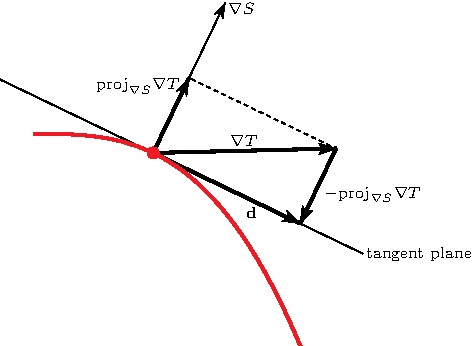
\includegraphics{OE14A_2.pdf}
\end{center}

The projection of $\vnabla T(0,-1,1)$ onto the normal vector
$\vnabla S(0,-1,1)$ is
\begin{align*}
\text{proj}_{\vnabla S(0,-1,1)}\vnabla T(0,-1,1)
&=\frac{\vnabla T(0,-1,1)\cdot \vnabla S(0,-1,1)}
         {|\vnabla S(0,-1,1)|^2}\vnabla S(0,-1,1) \\
&=\frac{\llt -1\,,\,0 \,,\,- 2\rgt\cdot \llt 1\,,\, -2 \,,\,3\rgt}
         {|\llt 1\,,\, -2 \,,\,3\rgt|^2}\llt 1\,,\, -2 \,,\,3\rgt \\
&=\frac{-7}{14}\llt 1\,,\, -2 \,,\,3\rgt
\end{align*}

So the optimal direction is
\begin{align*}
\vd&=\vnabla T(0,-1,1) -
\text{proj}_{\vnabla S(0,-1,1)}\vnabla T(0,-1,1) \\
&=\llt -1\,,\,0 \,,\,- 2\rgt
  -\frac{-7}{14}\llt 1\,,\, -2 \,,\,3\rgt \\
&= \llt -\frac{1}{2}\,,\,-1 \,,\,- \frac{1}{2}\rgt
\end{align*}
So any positive non zero multiple of $-\llt 1\,,\, 2\,,\,1\rgt$ will do.
Note, as a check, that $-\llt 1\,,\, 2\,,\,1\rgt$ has dot product zero,
i.e. is perpendicular to, $\vnabla S(0,-1,1)=\llt 1 \,,\, -2 \,,\, 3\rgt$.
\end{solution}

\begin{question}[M200 2014D] %1
Suppose that $f(x,y,z)$ is a function of three variables and let 
$\vu = \frac{1}{\sqrt{6}} \llt 1, 1, 2\rgt$ 
and $\vv = \frac{1}{\sqrt{3}} \llt 1, -1, -1\rgt$ 
and $\vw = \frac{1}{\sqrt{3}} \llt 1, 1, 1\rgt$. 
Suppose that at a point $(a,b,c)$,
\begin{align*}
D_\vu f&=0 \\
D_\vv f&=0 \\
D_\vw f&=4
\end{align*}
Find $\vnabla f$ at $(a,b,c)$.
\end{question}

%\begin{hint}
%
%\end{hint}

\begin{answer}
$\vnabla f(a,b,c) =\sqrt{3} \llt 2,6,-4\rgt$
\end{answer}

\begin{solution}
Write $\vnabla f(a,b,c) =\llt F,G,H\rgt$. We are told that
\begin{align*}
D_\vu f&=\frac{1}{\sqrt{6}} \llt 1, 1, 2\rgt \cdot \llt F,G,H\rgt = 0 \\
D_\vv f&=\frac{1}{\sqrt{3}} \llt 1, -1, -1\rgt \cdot \llt F,G,H\rgt = 0 \\
D_\vw f&=\frac{1}{\sqrt{3}} \llt 1, 1, 1\rgt \cdot \llt F,G,H\rgt = 4
\end{align*}
so that
\begin{align*}
 F + G + 2H &= 0 \tag{E1}\\
 F - G - H &= 0 \tag{E2}\\
 F + G + H &= 4\sqrt{3} \tag{E3}
\end{align*}
Adding (E2) and (E3) gives $2F=4\sqrt{3}$ or $F=2\sqrt{3}$.
Substituting $F=2\sqrt{3}$ into (E1) and (E2) gives
\begin{align*}
   G + 2H &= -2\sqrt{3} \tag{E1}\\
 - G - H &=  -2\sqrt{3} \tag{E2}
\end{align*}
Adding (E1) and (E2) gives $H=-4\sqrt{3}$ and substituting 
$H=-4\sqrt{3}$ back into (E2) gives $G=6\sqrt{3}$. All together
\begin{equation*}
\vnabla f(a,b,c) =\sqrt{3} \llt 2,6,-4\rgt
\end{equation*}
\end{solution}

%%%%%%%%%%%%%%%%%%%%%%%%%%%%%%%
\begin{question}[M200 2003D] %3
The elevation of a hill is given by the equation 
$f(x,y)=x^2y^2e^{-x-y}$. An ant sits at the point $(1,1,e^{-2})$.
\begin{enumerate}[(a)]
\item 
Find the unit vector $\vu=\llt u_1,u_2\rgt$ that maximizes
\begin{equation*}
\lim_{t\rightarrow 0}\frac{f\big((1,1)+t\vu\big)-f(1,1)}{t}
\end{equation*}

\item 
Find a vector $\vv=\llt v_1,v_2,v_3\rgt$ pointing in the direction
of the path that the ant could take in order to stay on the same elevation
level $e^{-2}$.

\item Find a vector $\vv=\llt v_1,v_2,v_3\rgt$ pointing in the direction
of the path that the ant should take in order to maximize its instantaneous
rate of level increase.
\end{enumerate}
\end{question}

%\begin{hint}
%
%\end{hint}

\begin{answer}
(a) $\frac{1}{\sqrt{2}}\llt 1,1\rgt$\qquad
(b) $\vv=c\llt 1,-1,0\rgt$ for any nonzero constant $c$

(c) $\vv=\frac{1}{\sqrt{2}}\llt 1,1,2e^{-2}\rgt$. Any positive multiple
of this vector is also a correct answer.
\end{answer}

\begin{solution}
(a) The expression
$
\lim_{t\rightarrow 0}\frac{f((1,1)+t\vu)-f(1,1)}{t}
$
is the directional derivative of $f$ at $(1,1)$ in the direction $\vu$,
which is $D_\vu f(1,1)=\vnabla f(1,1)\cdot\vu$. This is mazimized when $\vu$ is
parallel to  $\vnabla f(1,1)$. Since
\begin{equation*}
f_x(x,y)=2xy^2e^{-x-y}-x^2y^2e^{-x-y}\qquad
f_y(x,y)=2x^2ye^{-x-y}-x^2y^2e^{-x-y}
\end{equation*}
we have
\begin{equation*}
\vnabla f(1,1)=e^{-2}\llt 1,1\rgt
\end{equation*}
so that the desired unit vector $\vu$ is $\frac{1}{\sqrt{2}}\llt 1,1\rgt$.

(b) In order to remain at elevation $e^{-2}$, the ant must move so
that $D_\vu f(1,1)=0$. This is the case if $\vu\perp\vnabla f(1,1)$.
For example, we can take $\vu=\llt 1,-1\rgt$. When the ant moves 
in this direction, while remaining on the surface of the hill, its 
vertical component of velocity is zero. So $\vv=c\llt 1,-1,0\rgt$ for any 
nonzero constant $c$.

(c) In order to maximize its instantaneous rate of level increase,
the ant must choose the $x$ and $y$ coordinates of its velocity vector
in the same direction as  $\vnabla f(1,1)$. Namely $\vu=c\llt 1,1\rgt$ for any
$c>0$. To make $\vu$ a unit vector, we choose $c=\frac{1}{\sqrt{2}}$.
The corresponding value of the $z$ coordinate of its velocity vector is
the rate of change of $f$ per unit horizontal distance travelled, which
is the directional derivative 
\begin{equation*}
D_\vu f(1,1)=\vnabla f(1,1)\cdot\vu=e^{-2}\llt 1,1\rgt \cdot\llt c,c\rgt
=2ce^{-2}
\end{equation*}
 So $\vv=\frac{1}{\sqrt{2}}\llt 1,1,2e^{-2}\rgt$. Any positive multiple
of this vector is also a correct answer.
\end{solution}

%%%%%%%%%%%%%%%%%%%%%%%%%%%%%%%%
\begin{question}[M200 2001D] %3
Let the temperature in a region of space be given by 
$T(x,y,z)=3x^2+\half y^2+2z^2$ degrees.
\begin{enumerate}[(a)]
\item
A sparrow is flying along the curve $\vr(s)=\big(\frac{1}{3}s^3,2s,s^2\big)$
at a constant speed of $3{\rm ms}^{-1}$. What is the velocity of the sparrow
when $s=1$?

\item
At what rate does the sparrow feel the temperature is changing
at the point $A\big(\frac{1}{3},2,1\big)$ for which $s=1$.

\item
At the point $A\big(\frac{1}{3},2,1\big)$ in what direction
will the temperature be decreasing at maximum rate?

\item
 An eagle crosses the path of the sparrow 
at $A\big(\frac{1}{3},2,1\big)$, is moving at right angles to the path
of the sparrow, and is also moving in a direction in which the temperature
remains constant. In what directions could the eagle be flying as it passes
through the point $A$?
\end{enumerate}
\end{question}

%\begin{hint}
%
%\end{hint}

\begin{answer}
(a) $\llt 1,2,2\rgt$\qquad
(b) $14^\circ/{\rm s}$\qquad
(c) any positive constant times $-\llt 2,2,4\rgt$

(d) any positive constant times $\pm\llt 2,0,-1\rgt$
\end{answer}

\begin{solution}
(a) The direction of motion at $s=1$ is given by the tangent vector
\begin{equation*}
\vr'(s)=\llt s^2,2,2s\rgt\big|_{s=1}=\llt 1,2,2\rgt
\end{equation*}
Since the length of the velocity vector must be $3$,
\begin{equation*}
\text{velocity}=\vv=3\frac{\llt 1,2,2\rgt}{|\llt 1,2,2\rgt|}=\llt 1,2,2\rgt
\end{equation*}

(b) The rate of change of temperature per unit distance felt by the 
sparrow at $s=1$ is $\vnabla T\big(\frac{1}{3},2,1\big)\cdot\frac{\vv}{|\vv|}$.
 The rate of change of temperature per unit time felt by the 
sparrow at $s=1$ is
\begin{align*}
\vnabla T\left(\frac{1}{3},2,1\right)\cdot\frac{\vv}{|\vv|}\ |\vv|
&=\vnabla T\left(\frac{1}{3},2,1\right)\cdot\vv
=\vv\cdot\llt 6x,y,4z\rgt\Big|_{({1\over3},2,1\big)} \\
&=\llt 1,2,2\rgt\cdot\llt 2,2,4\rgt=14^\circ/{\rm s}
\end{align*}

(c) The temperature decreases at maximum rate in the direction
opposite the temperature gradient, which is (any positive constant times) $-\llt 2,2,4\rgt$.

(d) The eagle is moving at right angles to the direction of motion
of the sparrow, which is $\llt 1,2,2\rgt$. As the eagle is also moving 
in a direction for which the temperature remains constant, it must 
be moving perpendicularly to the temperature gradient, $\llt 2,2,4\rgt$. 
So the direction of the eagle must be (a posiitve constant times) 
one of
\begin{align*}
   \pm\llt 1,2,2\rgt \times\llt 2,2,4\rgt
=\pm\det\left[\begin{matrix}
                     \hi & \hj & \hk \\
                     1   &  2  & 2 \\
                     2   &  2  & 4
                \end{matrix}\right]
=\pm\llt 4,0,-2\rgt
\end{align*}
or equivalently, any positive constant times $\pm\llt 2,0,-1\rgt$.
\end{solution}

%%%%%%%%%%%%%%%%%%%%%%%%%%%%%%%%%%%%%%%%%
\begin{question} [M200 2001A] % 2
Assume that the temperature $T$ at a point $(x,y,z)$ near
a flame at the origin is given by 
\begin{equation*}
T(x,y,z)=\frac{200}{1+x^2+y^2+z^2}
\end{equation*}
where the coordinates are given in meters and the temperature is in degrees
Celsius. Suppose that at some moment in time, a moth is at the point $(3,4,0)$
and is flying at a constant speed of $1 {\rm m/s}$ in the direction of maximum
increase of temperature.
\begin{enumerate}[(a)]
\item 
Find the velocity vector $\vv$ of the moth at this moment.

\item
 What rate of change of temperature does the moth feel at that moment?
\end{enumerate}
\end{question}

%\begin{hint}
%
%\end{hint}

\begin{answer}
(a) $\vv=-\llt \frac{3}{5},\frac{4}{5},0\rgt$\qquad
(b) $\frac{500}{169}\approx 2.96^\circ/{\rm s}$
\end{answer}

\begin{solution}
(a) The moth is moving the direction of the temperature gradient
at $(3,4,0)$, which is
\begin{equation*}
\vnabla T(3,4,0)
=-200\frac{2x\hi+2y\hj+2z\hk}{{(1+x^2+y^2+z^2)}^2}\bigg|_{(3,4,0)}
=-400\frac{3\hi+4\hj}{26^2}
\end{equation*}
Since the speed of the moth is $1 {\rm m/s}$ its velocity vector is a vector
of length one in direction $-\frac{400}{26^2}\llt 3,4,0\rgt$ and hence is 
$\vv=-\frac{\llt 3,4,0\rgt}{|\llt 3,4,0\rgt|}
=-\llt\frac{3}{5},\frac{4}{5},0\rgt$.

(b) The rate of change of temperature (per unit time) the moth feels at 
that time is 
\begin{equation*}
\vnabla T(3,4,0)\cdot\vv
=\frac{400}{26^2}\llt 3,4,0\rgt\cdot \llt\frac{3}{5},\frac{4}{5},0\rgt
=\frac{400\times25}{26^2\times 5}
=\frac{500}{169}\approx 2.96^\circ/{\rm s}
\end{equation*}

\end{solution}

%%%%%%%%%%%%%%%%%%%%%%%%%%%%%%%%
\begin{question}[M200 2000D] %3
We say that $u$ is inversely proportional to $v$ if there
is a constant $k$ so that $u=k/v$. Suppose that the temperature $T$ in
a metal ball is inversely proportional to the distance from the centre
of the ball, which we take to be the origin. The temperature at the point
$(1,2,2)$ is $120^\circ$.
\begin{enumerate}[(a)]
\item
Find the constant of proportionality. 

\item
Find the rate of change of $T$ at $(1,2,2)$ in the direction
towards the point $(2,1,3)$.

\item
Show that at most points in the ball, the direction of greatest
increase is towards the origin.
\end{enumerate}
\end{question}

%\begin{hint}
%
%\end{hint}

\begin{answer}
(a) $360$\qquad
(b) $-\frac{40}{3\sqrt{3}}\approx-7.70$\qquad
(c) $\vnabla T(x,y,z)=-360\frac{x\hi+y\hj+z\hk}{{(x^2+y^2+z^2)}^{3/2}}$
\end{answer}

\begin{solution}
(a)
We are told that $T(x,y,z)=\frac{k}{|\llt x,y,z\rgt|}
=\frac{k}{\sqrt{x^2+y^2+z^2}}$ 
for some constant $k$ and that
\begin{equation*}
120=T(1,2,2)=\frac{k}{|\llt 1,2,2\rgt|}
\implies k=120\times\sqrt{1+2^2+2^2}
          = 360
\end{equation*}

(b) The (unit) direction from $(1,2,2)$ to $(2,1,3)$
is $\vd=\frac{\llt 2,1,3\rgt-\llt 1,2,2\rgt}{|\llt 2,1,3\rgt-\llt 1,2,2\rgt|}
=\frac{\llt 1,-1,1\rgt}{|\llt 1,-1,1\rgt|}=\frac{1}{\sqrt{3}}\llt 1,-1,1\rgt$. 
The desired rate of change of temperature is
\begin{align*}
D_{\vd} T(1,2,2)
&=\vnabla T(1,2,2)\cdot\vd
=-360\frac{x\hi+y\hj+z\hk}{{(x^2+y^2+z^2)}^{3/2}}\Big|_{\llt 1,2,2\rgt}\cdot\vd
\\
&=-360\frac{\llt 1,2,2\rgt}{27}\cdot\frac{\llt 1,-1,1\rgt}{\sqrt{3}}
=-\frac{40}{3\sqrt{3}}\approx-7.70
\end{align*}
degrees per unit distance.

(c) At $(x,y,z)$, the direction of greatest increase is in the direction
of the temperature gradient at $(x,y,z)$, which is 
$\vnabla T(x,y,z)
=-360\frac{x\hi+y\hj+z\hk}{{(x^2+y^2+z^2)}^{3/2}}$
and which points opposite to the radius vector. That is, it points towards
the origin. This argument only fails at $(x,y,z)=(0,0,0)$, where the gradient,
and indeed $T(x,y,z)$, is not defined.
\end{solution}

%%%%%%%%%%%%%%%%%%%%%%%%%%%%%%%%
\begin{question}[M200 2000A] %3
The depth of a lake in the $xy$-plane is equal to 
   $f(x, y) = 32-x^2-4x-4y^2$ meters. 
\begin{enumerate}[(a)]
\item
Sketch the shoreline of the lake in the $xy$-plane. 
\end{enumerate}
Your calculus instructor is in the water at the point $(-1, 1)$. 
Find a unit vector which indicates in which direction he should swim 
in order to: 
\begin{enumerate}[(a)]
\item[(b)] 
stay at a constant depth? 
\item[(c)]
increase his depth as rapidly as possible (i.e. be most likely to drown)? 
\end{enumerate}
\end{question}

%\begin{hint}
%
%\end{hint}

\begin{answer}
(a)
\begin{center}
     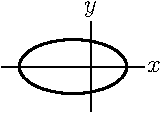
\includegraphics{OE00AQ3.pdf}
\end{center}

(b) $\pm\frac{1}{\sqrt{17}}\llt 4,-1\rgt$\qquad
(c) $-\frac{1}{\sqrt{17}}\llt 1,4\rgt$
\end{answer}

\begin{solution}
(a) The shoreline is $f(x,y)=0$ or $x^2+4x+4y^2=32$ or $(x+2)^2+4y^2=36$,
which is an ellipse centred on $(-2,0)$ with semiaxes $6$ in the $x$-direction
and $3$ in the $y$-direction.
\begin{center}
     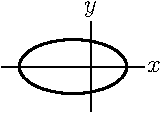
\includegraphics{OE00AQ3.pdf}
\end{center}

(b,c) The gradient of $f$ at $(-1,1)$ is
\begin{equation*}
\vnabla f(-1,1)=\big[(-2x-4)\,\hi-8y\,\hj\big]_{(-1,1)}=-2\,\hi-8\,\hj
\end{equation*}
To remain at constant depth, he should swim perpendicular to the depth
gradient. So he should swim in direction $\pm\frac{1}{\sqrt{17}}\llt 4,-1\rgt$.
To increase his depth as rapidly as possible, he should swim in the direction
of the depth gradient, which is $-\frac{1}{\sqrt{17}}\llt 1,4\rgt$.
\end{solution}

%%%%%%%%%%%%%%%%%%
\subsection*{\Application}
%%%%%%%%%%%%%%%%%%

%%%%%%%%%%%%%%%%%%%%%%%%%%%%%%%%
\begin{question}
The temperature $T(x,y)$ at points of the $xy$-plane is given by 
$T(x,y)=x^2-2y^2$.
\begin{enumerate}[(a)]
\item
Draw a contour diagram for $T$ showing some isotherms (curves
of constant temperature).
\item
In what direction should an ant at position $(2,-1)$ move if
it wishes to cool off as quickly as possible?
\item
If the ant moves in that direction at speed $v$ at what rate
does its temperature decrease?
\item
What would the rate of decrease of temperature of the ant be
if it moved from $(2,-1)$ at speed $v$ in direction $\llt -1,-2\rgt$?
\item
Along what curve through $(2,-1)$ should the ant move to continue
experiencing maximum rate of cooling?
\end{enumerate}
\end{question}

\begin{hint}
Review \S\eref{CLP200}{sec directional derivatives} in the CLP-3 text.

(e) Suppose that the ant moves along the curve $y=y(x)$. 
For the ant to always experience maximum rate of cooling (or maximum 
rate of heating), the tangent to this curve must be parallel to 
$\vnabla T(x,y)$ at every point of the curve. This gives a separable
differential equation for the function $y(x)$. Also, don't forget that $(2,-1)$ must be on the curve.
\end{hint}

\begin{answer}
(a) Here is a sketch which show the isotherms $T=0,\ 1,\ -1$ as well
as the branch of the $T=2$ isotherm that contains the ant's location
$(2,-1)$.
\begin{center}
     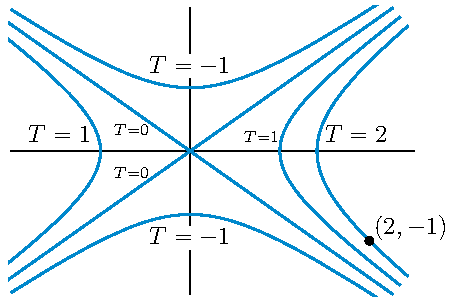
\includegraphics{ant.pdf}
\end{center}

(b) $\llt -1,-1\rgt/\sqrt{2}$\qquad
(c) $4\sqrt{2}\,v$\qquad
(d) $\frac{12}{\sqrt{5}}\,v$\qquad
(e) $y=-\frac{4}{x^2}$
\end{answer}

\begin{solution}
(a) The curve on which the temperature is $T_0$ is $x^2-2y^2=T_0$.
If $T_0=0$, this is the pair of straight lines $y=\pm\frac{x}{\sqrt{2}}$.
If $T_0>0$, it is a hyperbola on which $x^2=2y^2+T_0\ge T_0$.
If $T_0<0$, it is a hyperbola on which $2y^2=x^2-T_0\ge |T_0|$.
Here is a sketch which show the isotherms $T=0,\ 1,\ -1$ as well
as the branch of the $T=2$ isotherm that contains the ant's location
$(2,-1)$.
\begin{center}
     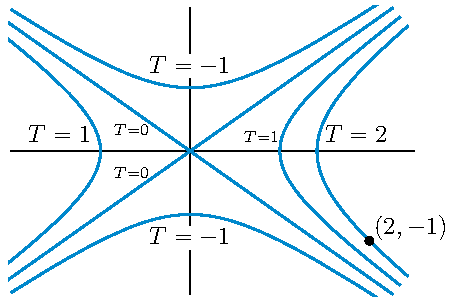
\includegraphics{ant.pdf}
\end{center}
Note that the temperature gradient is $\vnabla T(x,y)=\llt 2x,-4y\rgt$.
In particular, the temperature gradient at $(2,-1)$
is $\vnabla T(2,-1)=\llt 4,4\rgt$.

(b) To achieve maximum rate of cooling, the ant should move in the direction
opposite the temperature gradient at $(2,-1)$. So the direction of
maximum rate of cooling is 
\begin{equation*}
-\frac{\llt 4,4\rgt}{4\sqrt{2}}
    =\frac{\llt -1,-1\rgt}{\sqrt{2}}
\end{equation*}

(c) If the ant moves in the direction of part (b), its rate of cooling
per unit distance is $|\vnabla T(2,-1)|=|\llt 4,4\rgt| = 4\sqrt{2}$.
It the ant is moving at speed $v$, its rate of cooling
per unit time is $4\sqrt{2}\,v$.

(d) If the ant moves from $(2,-1)$  in direction $\llt -1,-2\rgt$
its temperature increases at the rate 
\begin{equation*}
  D_{\frac{\llt -1,-2\rgt}{\sqrt{5}}} T(2,-1)
        = \llt 4,4\rgt\cdot \frac{\llt -1,-2\rgt}{\sqrt{5}}
        = -\frac{12}{\sqrt{5}}
\end{equation*}
per unit distance. So, if the ant is moving at speed $v$,
its rate of decrease of temperature per unit time
is $\frac{12}{\sqrt{5}}\,v$



(e) Suppose that the ant moves along the curve $y=y(x)$. For the ant to always
experience maximum rate of cooling (or maximum rate of heating), 
the tangent to this curve must be parallel to $\vnabla T(x,y)$ at every point of the curve. A tangent to the curve at $(x,y)$ is $\llt 1,\diff{y}{x}(x)\rgt$.
This is parallel to $\vnabla T(x,y)=\llt 2x,-4y\rgt$ when
\begin{align*}
\frac{\diff{y}{x}}{1}=\frac{-4y}{2x}
\implies \frac{dy}{y}=-2\frac{dx}{x}
\implies \ln y=-2\ln x+C
\implies y=C'x^{-2}
\end{align*}
To pass through $(2,-1)$, we need $C'=-4$, so $y=-\frac{4}{x^2}$.

%If the ant is at $\big(x(t)sec directional derivatives,y(t)\big)$ at time $t$ and moves
%with constant speed, then the rate of cooling is 
%\begin{equation*}
%-\llt\diff{x}{t},\diff{y}{t}\rgt\cdot\vnabla T\big(x(t),y(t)\big)
%=-\llt\diff{x}{t},\diff{y}{t}\rgt\cdot\llt 2x,-4y\rgt
%\end{equation*}
%which is a maximum when $\llt\diff{x}{t},\diff{y}{t}\rgt
%\parallel \llt 2x,-4y\rgt$. This is the case when
%\begin{align*}
%\diff{y}{x}=\frac{\diff{y}{t}}{\diff{x}{t}}=\frac{4y}{-2x}
%\implies \frac{dy}{y}=-2\frac{dx}{x}
%\implies \ln y=-2\ln x+C
%\implies y=C'x^{-2}
%\end{align*}
%To pass through $(2,-1)$, we need $C'=-4$, so $y=-\frac{4}{x^2}$.


\end{solution}



%%%%%%%%%%%%%%%%%%%%%%%%%%%%%%%%
\begin{question}[M200 2008A] %3
Consider the function $f(x,y,z) = x^2 + \cos(yz)$.

\begin{enumerate}[(a)]
\item
Give the direction in which $f$ is increasing the fastest at the point 
$(1, 0, \pi/2)$.

\item
Give an equation for the plane $T$ tangent to the surface 
\begin{equation*}
S = \Set{(x,y,z)}{f(x,y,z) = 1}
\end{equation*}
at the point $(1, 0, \pi/2)$.

\item
Find the distance between $T$ and the point $(0, 1, 0)$.

\item
Find the angle between the plane $T$ and the plane
\begin{equation*}
P = \Set{(x,y,z)}{x + z = 0}.
\end{equation*}

\end{enumerate}
\end{question}

%\begin{hint}
%
%\end{hint}

\begin{answer}
(a) $\hi$\qquad
(b) $x=1$\qquad
(c) $1$\qquad
(d) $\frac{\pi}{4}$
\end{answer}

\begin{solution}
The first order partial derivatives of $f$, both at a general point 
$(x,y,z)$ and at the point $(1, 0, \pi/2)$, are
\begin{alignat*}{3}
f_x(x,y,z)&= 2x\qquad &
     f_x(1, 0, \pi/2)&= 2 \\
f_y(x,y,z)&= -z\sin(yz)\qquad &
     f_y(1, 0, \pi/2)&= 0 \\
f_z(x,y,z)&= -y\sin(yz)\qquad &
     f_z(1, 0, \pi/2)&= 0 
\end{alignat*}

(a) The rate of increase of $f$ is largest in the direction of 
$\vnabla f(1, 0, \pi/2)=\llt 2,0,0\rgt$. A unit vector in that direction
is $\hi$.

(b) The gradient vector $\vnabla f(1, 0, \pi/2)=\llt 2,0,0\rgt$ is a normal
vector to the surface $f=1$ at $(1, 0, \pi/2)$. So the specified tangent
plane is
\begin{align*}
\llt 2,0,0\rgt \cdot \llt x-1\,,\,y-0\,,\,z-\pi/2\rgt=0\qquad\text{or}\qquad
x=1
\end{align*} 

(c) The vector from the point $(0,1,0)$ to the point $(1,1,0)$, on $T$,
is $\llt 1,0,0\rgt$, which is perpendicular to $T$. So $(1,1,0)$
is the point on $T$ nearest $(0,1,0)$  and the distance from $(0,1,0)$ to $T$
is $|\llt 1,0,0\rgt|=1$.

(d) The vector $\llt 1,0,1\rgt$ is perpendicular to the plane $x+z=0$.
So the angle between the planes $T$ and $x+z=0$ is the same as the angle
$\theta$ between the vectors $\llt 1,0,0\rgt$ and $\llt 1,0,1\rgt$,
which obeys
\begin{align*}
& |\llt 1,0,0\rgt| \ |\llt 1,0,1\rgt|\ \cos\theta 
   =|\llt 1,0,0\rgt\cdot\llt 1,0,1\rgt| 
   =1 \\
&\implies \cos\theta=\frac{1}{\sqrt{2}}
\implies  \theta=\frac{\pi}{4} 
\end{align*}
\end{solution}

%%%%%%%%%%%%%%%%%%%%%%%%%%%%%%%%
\begin{question}[M200 2015D] %2
A function $T(x,y,z)$ at $P = (2,1,1)$ is known to have 
$T(P) = 5$, $T_x (P) = 1$, $T_y(P) = 2$, and $T_z(P) = 3$.
\begin{enumerate}[(a)]
\item
A bee starts flying at $P$ and flies along the unit vector pointing 
towards the point $Q = (3,2,2)$. What is the rate of change of 
$T(x,y,z)$ in this direction?
\item
Use the linear approximation of $T$ at the point $P$ to approximate 
$T(1.9,1,1.2)$.
\item
Let $S(x,y,z) = x + z$. A bee starts flying at $P$; along which unit 
vector direction should the bee fly so that the rate of change of $T(x,y,z)$ 
and of $S(x,y,z)$ are both zero in this direction?
\end{enumerate}
\end{question}

%\begin{hint}
%
%\end{hint}

\begin{answer}
(a) $2\sqrt{3}$ \qquad
(b) $5.5$\qquad
(c) $\pm\frac{\llt 1,1,-1\rgt}{\sqrt{3}}$
\end{answer}

\begin{solution}
(a) We are being asked for the directional derivative of
$T$ in the direction of the  unit vector from $P=(2,1,1)$ to $Q=(3,2,2)$, 
which is $\frac{\llt 1,1,1\rgt}{\sqrt{3}}$. That directional
derivative is
\begin{align*}
\vnabla T(P)\cdot \frac{\llt 1,1,1\rgt}{\sqrt{3}}
=\llt 1,2,3\rgt \cdot \frac{\llt 1,1,1\rgt}{\sqrt{3}}
=2\sqrt{3}
\end{align*}

(b) The linear approximation to $T$ at $P$ is
\begin{align*}
T(2+\De x\,,\,1+\De y\,,\,1+\De z)
   &\approx T(P) + T_x(P)\,\De x + T_y(P)\,\De y + T_z(P)\,\De z \\
   &= 5 +\De x +2\,\De y +3\,\De z 
\end{align*}
Applying this with $\De x = -0.1$, $\De y = 0$, $\De z=0.2$ gives
\begin{align*}
T(1.9\,,\,1\,,\,1.2)
   &\approx 5 +(-0.1) +2\,(0) +3\,(0.2) 
   =5.5
\end{align*}

(c) For the rate of change of $T$ to be zero, the direction of
motion must be perpendicular to $\vnabla T(P) = \llt 1,2,3\rgt$.
For the rate of change of $S$ to also be zero, the direction of
motion must also be perpendicular to $\vnabla S(P) = \llt 1,0,1\rgt$.
The vector 
\begin{align*}
\llt 1,2,3\rgt \times \llt 1,0,1\rgt
&=\det\left[\begin{matrix}
             \hi & \hj & \hk\\ 
              1  &  2  & 3 \\
              1  &  0  & 1\end{matrix}\right]
=\llt 2,2,-2\rgt
\end{align*}
is perpendicular to both $\vnabla T(P)$ and $\vnabla S(P)$.
So the desired unit vectors are $\pm\frac{\llt 1,1,-1\rgt}{\sqrt{3}}$.
\end{solution}

%%%%%%%%%%%%%%%%%%%%%%%%%%%%%%%%
\begin{question}[M200 2016D] %3
Consider the functions $F(x,y,z) = z^3 +xy^2 +xz$ and $G(x,y,z)=3x-y+4z$.
You are standing at the point $P(0,1,2)$.
\begin{enumerate}[(a)]
\item
You jump from $P$ to $Q(0.1\,,\,0.9\,,\,1.8)$. Use the linear approximation
to determine approximately the amount by which $F$ changes.

\item
You jump from $P$ in the direction along which $G$ increases most rapidly.
Will $F$ increase or decrease?

\item
You jump from $P$ in a direction $\llt a\,,\,b\,,\,c\rgt$ along which the rates 
of change of $F$ and $G$ are both zero. Give an example of such a direction
(need not be a unit vector).

\end{enumerate}
\end{question}

%\begin{hint}
%
%\end{hint}

\begin{answer}
(a) $-2.1$\qquad
(b) $F$ increases.\qquad
(c) Any nonzero constant times $\llt 4 \,,\, 8 \,,\, -1 \rgt$.
\end{answer}

\begin{solution}
We are going to need the gradients of both $F$ and $G$ at $(0,1,2)$. 
So we compute
\begin{align*}
\pdiff{F}{x}(x,y,z)&=y^2+z &
\pdiff{F}{y}(x,y,z)&=2xy  &
\pdiff{F}{z}(x,y,z)&=3z^2+x \\
\pdiff{G}{x}(x,y,z)&=3 &
\pdiff{G}{y}(x,y,z)&=-1  &
\pdiff{G}{z}(x,y,z)&=4
\end{align*}
and then
\begin{equation*}
\vnabla F(0,1,2) = \llt 3,0,12 \rgt\qquad
\vnabla G(0,1,2) = \llt 3,-1,4 \rgt
\end{equation*}

(a) The linear approximation to $F$ at $(0,1,2)$ is
\begin{align*}
F(x,y,z) 
&\approx F(0,1,2) + F_x(0,1,2)\,x + F_y(0,1,2)\,(y-1) + F_z(0,1,2)\,(z-2) \\
&=8+ 3 x + 12 (z-2)
\end{align*}
In particular
\begin{align*}
F(0.1\,,\,0.9\,,\,1.8) - F(0,1,2)
&\approx 3(0.1) + 12(-0.2)
=-2.1
\end{align*}

(b) The direction along which $G$ increases most rapidly at $P$ is
$\vnabla G(0,1,2) = \llt 3,-1,4 \rgt$. The directional derivative of $F$
in that direction is
\begin{align*}
D_{\frac{\llt 3,-1,4\rgt}{\sqrt{26}}}F(0,1,2) 
 = \vnabla F(0,1,2) \cdot \frac{\llt 3,-1,4\rgt}{\sqrt{26}}
 = \llt 3,0,12 \rgt\cdot \frac{\llt 3,-1,4\rgt}{\sqrt{26}}
 > 0
\end{align*}
So $F$ increases.

(c) 
For the rate of change of $F$ to be zero, 
$\llt a\,,\,b\,,\,c\rgt$ must be perpendicular to 
$\vnabla F(0,1,2) = \llt 3,0,12  \rgt$.

For the rate of change of $G$ to be zero, 
$\llt a\,,\,b\,,\,c\rgt$ must be perpendicular to 
$\vnabla G(0,1,2) = \llt 3,-1,4 \rgt$.

So any nonzero constant times
\begin{align*}
\det\left[\begin{matrix}
            \hi  &  \hj  &  \hk \\
            3    &   0   &   12 \\
            3    &  -1   &    4 
            \end{matrix}\right]
=\llt 12 \,,\, 24 \,,\, -3 \rgt
=3 \llt 4 \,,\, 8 \,,\, -1 \rgt
\end{align*}
is an allowed direction.
\end{solution}

%%%%%%%%%%%%%%%%%%%%%%%%%%%%%%%%
\begin{question}[M200 2004A] %3
A meteor strikes the ground in the heartland of Canada. 
Using satellite photographs, a model
\begin{equation*}
z=f(x,y)=-\frac{100}{x^2+2x+4y^2+11}
\end{equation*}
of the resulting crater is made and a plan is drawn up to convert the site into
a tourist attraction. A car park is to be built at  $(4,5)$ and a hiking trail is to be made. The trail is to start at the car park and take the steepest route to the bottom of the crater.
\begin{enumerate}[(a)]
\item
  Sketch a map of the proposed site clearly marking the car park, 
a few level curves for the function $f$  and the trail.

\item  
In which direction does the trail leave the car park? 
\end{enumerate}
\end{question}

%\begin{hint}
%
%\end{hint}

\begin{answer}
(a) \begin{center}
     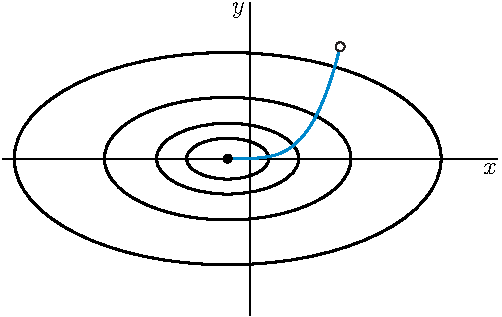
\includegraphics{crater.pdf}
\end{center}

(b) $-\llt 1,4\rgt$

\end{answer}

\begin{solution}
(a)  Since
\begin{equation*}
z=-\frac{100}{x^2+2x+4y^2+11}=-\frac{100}{(x+1)^2+4y^2+10}
\end{equation*}
the bottom of the crater is at $x=-1$, $y=0$ (where the denominator is
a minimum) and the contours (level curves) are ellipses having equations
$(x+1)^2+4y^2=C$. In the sketch below, the filled dot represents the 
bottom of the crater and the open dot represents the car park. The 
contours sketched are (from inside out) $z=-7.5, -5, -2.5, -1$. Note that
the trail crosses the contour lines at right angles.

\begin{center}
     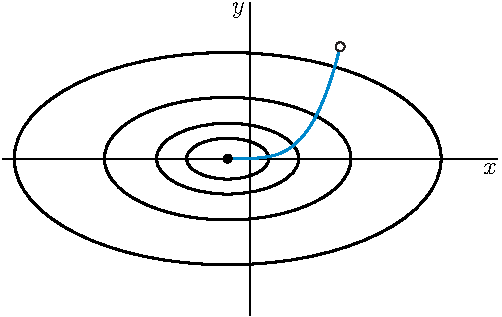
\includegraphics{crater.pdf}
\end{center}

(b) The trail is to be parallel to 
$$
\vnabla z = \frac{100}{{(x^2+2x+4y^2+11)}^2}(2x+2,8y)
$$
At the car park $\vnabla z(4,5)\parallel \llt 10, 40\rgt\parallel \llt 1,4\rgt$.
To move towards the bottom of the crater, we should leave in the direction  
$-\llt 1,4\rgt$.
\end{solution}

%%%%%%%%%%%%%%%%%%%%%%%%%%%%%%%%%%%%%%%%%
\begin{question} [M200 2002D] % 3
 You are standing at a lone palm tree in the middle of the
Exponential Desert. The height of the sand dunes around you is given in
meters by 
$$
h(x,y)=100 e^{-(x^2+2y^2)}
$$
where $x$ represents the number of meters east of the palm tree (west if
$x$ is negative) and $y$ represents the number of meters north of the palm
tree (south if $y$ is negative).
\begin{enumerate}[(a)]
\item 
Suppose that you walk $3$ meters east and 2 meters north.
At your new location, $(3,2)$, in what direction is the sand dune sloping
most steeply downward?

\item
If you walk north from the location described in part (a),
what is the instantaneous rate of change of height of the sand dune?

\item
 If you are standing at $(3,2)$ in what direction should you
walk to ensure that you remain at the same height?

\item
 Find the equation of the curve through $(3,2)$ that you should
move along in order that you are always pointing in a steepest descent
direction at each point of this curve.
\end{enumerate}
\end{question}

%\begin{hint}
%
%\end{hint}

\begin{answer}
(a) any positive multiple of $\llt 3,4\rgt$\qquad
(b) $-800 e^{-17}$\qquad
(c) $\pm\big(\frac{4}{5},-\frac{3}{5}\big)$\qquad
(d) $y=\frac{2}{9}x^2$
\end{answer}

\begin{solution}
We have
\begin{equation*}
\vnabla h(x,y)= -200 e^{-(x^2+2y^2)}\llt x,2y\rgt\text{ and, in particular, }
\vnabla h(3,2)= -200 e^{-17}\llt 3,4\rgt
\end{equation*}

(a) At $(3,2)$ the dune slopes downward the most steeply in the direction
opposite $\vnabla h(3,2)$, which is (any positive multiple of) $\llt 3,4\rgt$.

(b) The rate is $D_{\hj} h(3,2)=\vnabla h(3,2)\cdot\hj=-800 e^{-17}$.

(c) To remain at the same height, you should walk perpendicular to
$\vnabla h(3,2)$. So you should walk in one of the directions 
$\pm\big(\frac{4}{5},-\frac{3}{5}\big)$.

(d) Suppose that you are walking along a steepest descent curve.
Then the direction from $(x,y)$ to $(x+\dee{x}, y+\dee{y})$, with 
$(\dee{x},\dee{y})$ infinitesmal, must be opposite to 
$\vnabla h(x,y)= -200 e^{-(x^2+2y^2)}(x,2y)$.
Thus $(\dee{x},\dee{y})$ must be parallel to $(x,2y)$ so that the slope
\begin{align*}
\diff{y}{x}=\frac{2y}{x}
\implies \frac{\dee{y}}{y}=2\frac{\dee{x}}{x}
\implies \ln y=2\ln x+C
\end{align*}
We must choose $C$ to obey $\ln 2=2\ln 3+C$ in order to pass through 
the point $(3,2)$. Thus $C=\ln\frac{2}{9}$ and the curve is 
$\ln y=2\ln x+\ln\frac{2}{9}$ or $y=\frac{2}{9}x^2$.
\end{solution}

%%%%%%%%%%%%%%%%%%%%%%%%%%%%%%%%
\begin{question}[M200 2002A] %4
Let $f(x,y)$ be a differentiable function with $f(1,2)=7$. Let
\begin{equation*}
\vu=\frac{3}{5}\,\hi+\frac{4}{5}\,\hj,\qquad
\vv=\frac{3}{5}\,\hi-\frac{4}{5}\,\hj
\end{equation*}
be unit vectors. Suppose it is known that the directional derivatives 
$D_\vu f(1,2)$ and $D_\vv f(1,2)$ are equal to $10$ and $2$ respectively.
\begin{enumerate}[(a)]
\item
Show that the gradient vector $\vnabla f$ at $(1,2)$ is $10\hi+5\hj$.

\item 
Determine the rate of change of $f$ at $(1,2)$ in the direction
of the vector $\hi+2\hj$.

\item 
Using the tangent plane approximation, estimate the value
of $f(1.01,2.05)$.
\end{enumerate}
\end{question}

%\begin{hint}
%\end{hint}

\begin{answer}
(a) See the solution.\qquad
(b) $4\sqrt{5}\approx 8.944$\qquad
(c) $7.35$
\end{answer}

\begin{solution}
(a)
Denote $\vnabla f(1,2)= \llt a,b\rgt$. We are told that
\begin{alignat*}{3}
D_\vu f(1,2)&=\vu\cdot(a,b)&&=\frac{3}{5}a+\frac{4}{5}b&&=10 \\
D_\vv f(1,2)&=\vv\cdot(a,b)&&=\frac{3}{5}a-\frac{4}{5}b&&=2
\end{alignat*}
Adding these two equations gives $\frac{6}{5}a=12$, which forces $a=10$,
and subtracting the two equations gives $\frac{8}{5}b=8$, which forces
$b=5$, as desired.

(b) The rate of change of $f$ at $(1,2)$ in the direction
of the vector $\hi+2\hj$ is
\begin{align*}
\frac{\hi+2\hj}{|\hi+2\hj|}\cdot \vnabla f(1,2)
=\frac{1}{\sqrt{5}}\llt 1,2\rgt\cdot\llt 10,5\rgt
=4\sqrt{5}\approx 8.944
\end{align*}

(c) Applying (\eref{CLP200}{eqn lin approx 2d} in the CLP3 text, which is
\begin{align*}
f\big(x_0+\De x\,,\,y_0+\De y\big)
&\approx f\big(x_0\,,\,y_0\big) 
       + \pdiff{f}{x}\big(x_0\,,\,y_0\big)\,\De x
       + \pdiff{f}{y}\big(x_0\,,\,y_0\big)\,\De y
\end{align*}
with $x_0=1$, $\De x=0.01$, $y_0=2$, and $\De y=0.05$, gives
\begin{align*}
f(1.01,2.05)
&\approx f(1,2)+f_x(1,2)\times(1.01-1)+f_y(1,2)\times(2.05-2) \\
&=7+10\times0.01+5\times0.05 \\
&=7.35
\end{align*}
\end{solution}

